\documentclass[tikz,border=2pt]{standalone}
\usepackage{amsmath,amssymb,bm}
\usetikzlibrary{arrows.meta,positioning,fit}
\begin{document}
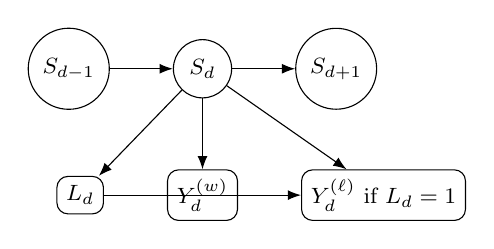
\begin{tikzpicture}[>=Latex, node distance=9mm and 8mm, every node/.style={font=\footnotesize}]
\node[draw,circle,minimum size=7mm] (s1) {$S_{d-1}$};
\node[draw,circle,minimum size=7mm,right=of s1] (s2) {$S_d$};
\node[draw,circle,minimum size=7mm,right=of s2] (s3) {$S_{d+1}$};
\draw[->] (s1)--(s2); \draw[->] (s2)--(s3);
\node[draw,rectangle,rounded corners,below=of s2] (w) {$Y_d^{(w)}$};
\node[draw,rectangle,rounded corners,left=of w] (l) {$L_d$};
\node[draw,rectangle,rounded corners,right=of w] (b) {$Y_d^{(\ell)}$ if $L_d=1$};
\draw[->] (s2)--(w); \draw[->] (s2)--(l); \draw[->] (s2)--(b);
\draw[->] (l)--(b);
\end{tikzpicture}
\end{document}
